\ylDisplay{Kiilud} % Ülesande nimi
{Tundmatu autor} % Autor
{lahtine} % Voor
{2006} % Aasta
{G 6} % Ülesande nr.
{5} % Raskustase
{
% Teema: Geomeetriline-optika
\ifStatement
Tasaparalleelne plaat koosneb kahest klaaskiilust väikse nurgaga $\varphi \ll 1$ (vt joonist). Kiilude murdumisnäitajad on $n_1$ ja $n_2$ ($n_2 > n_1$). Plaadile risti tema pinnaga langeb paralleelne valgusvihk. Plaadi taga asub koondav lääts fookuskaugusega $f$. Läätse fokaaltasandis asub ekraan. Joonistage kiirte käik süsteemis. Kui palju nihkub valguslaik ekraanil, kui me eemaldame plaadi? 

\emph{Vihje}. Väikeste nurkade puhul kehtib ligikaudne võrdus $\tan \varphi \approx \sin \varphi \approx \varphi $.

\begin{center}
	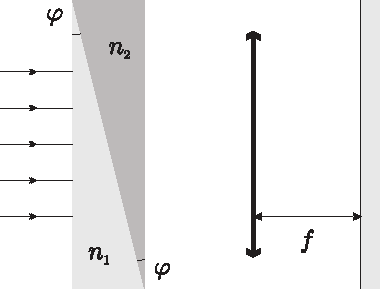
\includegraphics[width=0.6\linewidth]{2006-lahg-06-yl}
\end{center}
\fi


\ifHint
On lihtne näha, et plaadist väljub endiselt paralleelne valgusvihk. Küll aga on selle levimise suund muutunud. Valguslaigu nihke leidmiseks on mugav vaadelda kiirt, mis läbib läätse optilist keskpunkti.
\fi


\ifSolution
On lihtne näha, et plaadist väljub endiselt paralleelne valgusvihk. Küll aga on selle levimise suund muutunud. Plaati sisenedes murdumist ei toimu, sest kiired liiguvad risti pinnaga. Kaldpinnale langevad kiired langemisnurga $\varphi$ all, murdumisnurga $\gamma$ saame murdumisseadusest:
\[
n_1 \sin \varphi = n_2 \sin \gamma.
\]
Meil on lubatud kasutada väikeste nurkade lähendust $\sin \alpha \approx \alpha$, mistõttu $\varphi n_1 = \gamma n_2$. Murdumise tõttu muutus kiirte levimise suund nurga $\varphi -\gamma$ võrra. Ühtlasi on lihtne näha, et see on ka langemisnurgaks plaadi välistasandile, sest esialgu liikus kiir risti plaadiga. Arvestades, et õhu murdumisnäitaja on 1, saame leida kiire murdumisnurga $\delta$ plaadist väljumisel:
\[
n_{2}(\varphi-\gamma)=\delta, \quad \delta=n_{2}\left(\varphi-\frac{\varphi n_{1}}{n_{2}}\right)=\varphi\left(n_{2}-n_{1}\right).
\]
Valguslaigu nihet on nüüd lihtne leida. Vaatleme läätse optilist keskpunkti
läbivat kiirt. Et see kiir läätses ei murdu, lõikab see fokaaltasandit teljest kaugusel
\[
d = \delta f = \varphi f (n_2 - n_1).
\]
\fi
}